\newpage
\texHeader

Now, lets think about this whole Text Syntax. How exactly does it work? How will we be able to generate Java code from our simplified model code?

As you now know, Emoflon is an plug-in tool for Eclipse. More precisely, EMoflon needs the the Eclipse Modeling Framework (EMF) in order to work. EMF is comprised of two separate Metamodels - Genmodel and Ecore. The Genmodel contains the boring information about code generation like path and file information. 
We are more interested in Ecore, which we represent through our MOSL syntax. 

When you switched the project explorer from ``Projects" to ``Top Level Elements," you noticed that a few new nodes were created. Each node you see has a different criteria for grouping related Eclipse Projects together, which makes them your project ``Working Sets.'' The ``Specification'' node contains all the metamodels projects in a workspace (Fig. ~\ref{fig_modelSpecification}). That means, for every new Metamodel you create in your current workspace, all of the text code will be placed here. 

 \begin{figure}[htbp]
  \centering
  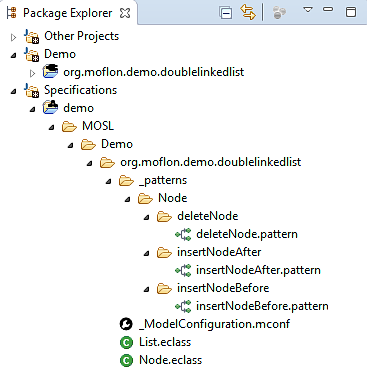
\includegraphics[width=0.5\textwidth]{eclipse_Specification}
  \caption{Eclipse: Specification Working Set}
  \label{fig_modelSpecification}
\end{figure}
  

Instead, lets look at the two eclass files and their syntax. Expand the folders, and you'll see that each eclass is declared in its own file. While you can combine several class delcarations in a single file in some languages (like Java), with MOSL it really is best to have them separated. It'll all make sense in a moment when we discuss Patterns.

Inspect the ``List'' class, and you'll see it has a just one EAttribute. EAttributes are defined by their name followed by a colon symbol and type.
This class also has a container reference represented by the diamond operator in front of an arrow.
The second reference type is a simple reference which